\documentclass[aspectratio=169,10pt]{beamer}

\usepackage[T2A]{fontenc}
\usepackage[utf8]{inputenc}
\usepackage[english,russian]{babel}
\usepackage{array}
\usepackage{booktabs}
\usepackage{graphicx}
\usepackage{tabularx}

\usetheme{Boadilla}
\usecolortheme{seahorse}
\setbeamertemplate{navigation symbols}{}
\setbeamertemplate{caption}[numbered]
\setbeamertemplate{footline}[frame number]

\definecolor{ThesisBlue}{RGB}{36, 82, 133}
\definecolor{ThesisGreen}{RGB}{47, 122, 91}
\definecolor{ThesisRed}{RGB}{158, 64, 54}
\setbeamercolor{title}{fg=ThesisBlue}
\setbeamercolor{frametitle}{fg=ThesisBlue}
\setbeamercolor{structure}{fg=ThesisBlue}
\setbeamercolor{block title}{fg=white,bg=ThesisBlue}
\setbeamercolor{block body}{fg=black,bg=ThesisBlue!6}

\graphicspath{{images/}}

\newcolumntype{Y}{>{\raggedright\arraybackslash}X}
\newcommand{\metric}[1]{\textcolor{ThesisBlue}{\textbf{#1}}}
\newcommand{\limitnote}[1]{\textcolor{ThesisRed}{#1}}

\title[Реконструкция визуальных стимулов по EEG]{Реконструкция визуальных стимулов на основе многоканальных EEG методами машинного обучения}
\author{Кошман Вячеслав Владимирович}
\institute{09.04.01 Информатика и вычислительная техника\\Профиль: Робототехника и компьютерное зрение}
\date{2026}

\begin{document}

\begin{frame}[plain]
  \vspace{0.8em}
  \begin{center}
    {\Large\textcolor{ThesisBlue}{\textbf{Реконструкция визуальных стимулов}}}

    \vspace{0.35em}
    {\large\textcolor{ThesisBlue}{на основе многоканальных EEG методами машинного обучения}}

    \vspace{1.8em}
    {\large Кошман Вячеслав Владимирович}

    \vspace{1.1em}
    \small
    09.04.01 Информатика и вычислительная техника\\
    Профиль: Робототехника и компьютерное зрение

    \vspace{1.8em}
    Научный руководитель: д.ф.-м.н. Максименко Владимир Александрович

    \vfill
    2026
  \end{center}
\end{frame}

\begin{frame}{Актуальность и сложность задачи}
  \begin{columns}[T,totalwidth=\textwidth]
    \begin{column}{0.54\textwidth}
      \begin{itemize}
        \item Visual imagery не имеет внешнего сенсорного ответа как при perception.
        \item EEG имеет высокое временное, но низкое пространственное разрешение.
        \item Малый корпус и повторные пробы требуют строгой оценки без утечек.
      \end{itemize}
      \begin{block}{Научный вопрос}
        Достаточно ли информации в EEG фазы воспоминания, чтобы восстановить структуру образа по отдельным пикселям?
      \end{block}
    \end{column}
    \begin{column}{0.42\textwidth}
      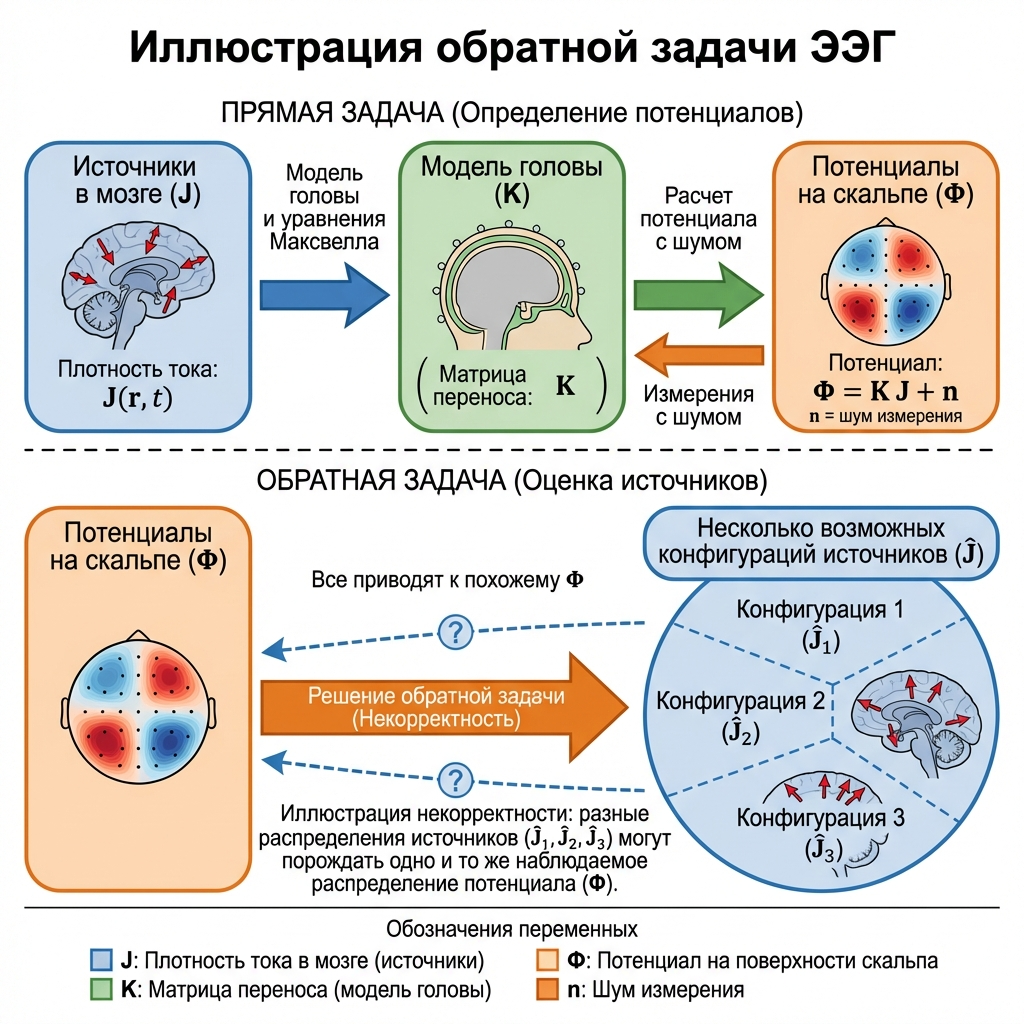
\includegraphics[width=\linewidth]{eeg_forward_inverse_problem.png}
    \end{column}
  \end{columns}
\end{frame}

\begin{frame}{Цель и задачи работы}
  \begin{block}{Цель}
    Разработать и исследовать воспроизводимый контур реконструкции бинарных визуальных стимулов $6\times6$ по EEG в фазе воспоминания при строгом контроле утечек.
  \end{block}
  \begin{columns}[T,totalwidth=\textwidth]
    \begin{column}{0.47\textwidth}
      \begin{block}{Объект}
        EEG-сигналы фазы воспоминания и связанные с ними бинарные изображения $6\times6$.
      \end{block}
    \end{column}
    \begin{column}{0.47\textwidth}
      \begin{block}{Предмет}
        Признаковые, спектральные и нейросетевые представления для реконструкции пикселей.
      \end{block}
    \end{column}
  \end{columns}
  \vspace{0.4em}
  \small
  \begin{itemize}
    \item Сформулировать задачу как 36 бинарных выходов и подготовить входы EEG.
    \item Сравнить классические модели, спектральные представления и компактные CNN.
    \item Оценить переносимость в разных протоколах с bootstrap-неопределенностью.
  \end{itemize}
\end{frame}

\begin{frame}{Постановка: реконструкция вместо классификации}
  \begin{columns}[T,totalwidth=\textwidth]
    \begin{column}{0.52\textwidth}
      \[
        X_i \in \mathbb{R}^{C \times T}
        \quad \rightarrow \quad
        \hat{\mathbf y}_i \in \{0,1\}^{36}
      \]
      \begin{itemize}
        \item Вход: многоканальный EEG-фрагмент.
        \item Выход: 36 оценок активности пикселей.
        \item Решение: пороговая бинаризация в изображение $6\times6$.
        \item Это не выбор класса, а восстановление локальной структуры стимула.
      \end{itemize}
    \end{column}
    \begin{column}{0.40\textwidth}
      \centering
      \setlength{\tabcolsep}{4pt}
      \renewcommand{\arraystretch}{1.25}
      \begin{tabular}{|c|c|c|c|c|c|}
        \hline
        0 & 1 & 0 & 0 & 1 & 0 \\ \hline
        1 & 1 & 0 & 0 & 0 & 1 \\ \hline
        0 & 0 & 1 & 1 & 0 & 0 \\ \hline
        0 & 1 & 1 & 0 & 1 & 0 \\ \hline
        1 & 0 & 0 & 1 & 0 & 1 \\ \hline
        0 & 0 & 1 & 0 & 1 & 0 \\ \hline
      \end{tabular}
    \end{column}
  \end{columns}
\end{frame}

\begin{frame}{Данные и экспериментальная подвыборка}
  \begin{tabularx}{\textwidth}{@{}lY@{}}
    \toprule
    Уровень & Содержание \\
    \midrule
    Исходный корпус & 16 испытуемых, 31 экспериментальная проба, 651 синхронизированное EEG / eye-tracking наблюдение. \\
    Типы стимулов & 434 геометрических и 217 случайных наблюдений в исходном описании. \\
    Основной эксперимент & 180 наблюдений случайных стимулов фазы воспоминания, одно наблюдение -- одна строка модели. \\
    Вход модели & Только EEG-каналы; EOG сохраняется как контекст и контроль качества, но не входит в признаки. \\
    \bottomrule
  \end{tabularx}
  \vspace{0.8em}
  \begin{block}{Единица анализа}
    Для признаковых и спектральных представлений используется интервал $[0.5, 15.5)$ с, приведенный к 125 Гц. Полное 15-секундное окно соответствует одному целевому изображению.
  \end{block}
\end{frame}

\begin{frame}{Воспроизводимый контур оценки без утечек}
  \centering
  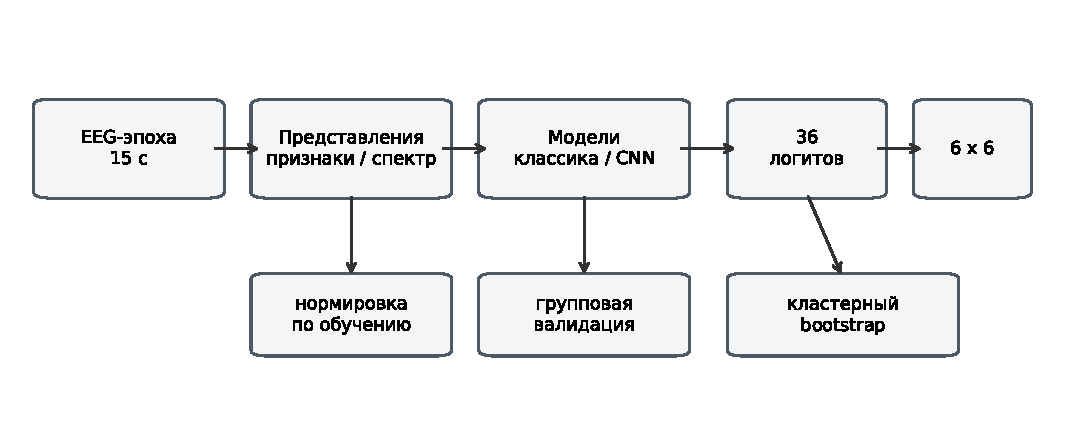
\includegraphics[width=0.86\textwidth,height=0.46\textheight,keepaspectratio]{experiment_pipeline.pdf}

  \vspace{0.5em}
  \begin{columns}[T,totalwidth=\textwidth]
    \begin{column}{0.32\textwidth}
      \small Разбиения учитывают испытуемых, пробы, ключи примеров и полные целевые изображения.
    \end{column}
    \begin{column}{0.32\textwidth}
      \small Признаки, нормализация, отбор и гиперпараметры настраиваются только по обучающей части.
    \end{column}
    \begin{column}{0.32\textwidth}
      \small Метрики, предсказания, bootstrap и инвентарь артефактов сохраняются для проверки.
    \end{column}
  \end{columns}
\end{frame}

\begin{frame}{Представления сигнала и модели}
  \begin{tabularx}{\textwidth}{@{}lY@{}}
    \toprule
    Компонент & Что сравнивалось \\
    \midrule
    Ручные признаки & Временные статистики, спектральные мощности, пространственные ковариации, LNDP / 1D-LGP / 1D-LBP. \\
    Спектральные входы & FFT/Welch как канал--частота; Morlet, Superlet и STFT как канал--частота--время. \\
    Классические модели & Logistic Regression как референс; SVM, Ridge, ElasticNet/Lasso, Random Forest, PLS. \\
    Нейросетевые модели & 12 вариантов: EEGNet, DeepConvNet и ShallowConvNet на четырех спектральных представлениях. \\
    \bottomrule
  \end{tabularx}
  \vspace{0.8em}
  \small Все обучаемые этапы подбираются внутри обучающей части соответствующего протокола.
\end{frame}

\begin{frame}{Протоколы и метрики оценки}
  \begin{tabularx}{\textwidth}{@{}lYY@{}}
    \toprule
    Протокол & Что проверяет & Размеры \\
    \midrule
    Межсубъектный & Перенос на новых испытуемых без пересечения субъектов между обучением и тестом. & 141 обучение / 39 тест. \\
    Двунаправленный межпробный & Перенос между пробами при совпадающих испытуемых, но разных пробах и целях. & 81 обучение / 81 тест в каждом направлении. \\
    \bottomrule
  \end{tabularx}
  \vspace{0.7em}
  \begin{columns}[T,totalwidth=\textwidth]
    \begin{column}{0.48\textwidth}
      \small Главная метрика: balanced accuracy по 36 пиксельным задачам; случайный ориентир \metric{0.5}.
    \end{column}
    \begin{column}{0.48\textwidth}
      \small Неопределенность: субъектно-кластерный bootstrap; сравнения с Logistic Regression через парный bootstrap и поправку Holm.
    \end{column}
  \end{columns}
\end{frame}

\begin{frame}{Результаты реконструкции: близко к случайному уровню}
  \begin{columns}[T,totalwidth=\textwidth]
    \begin{column}{0.48\textwidth}
      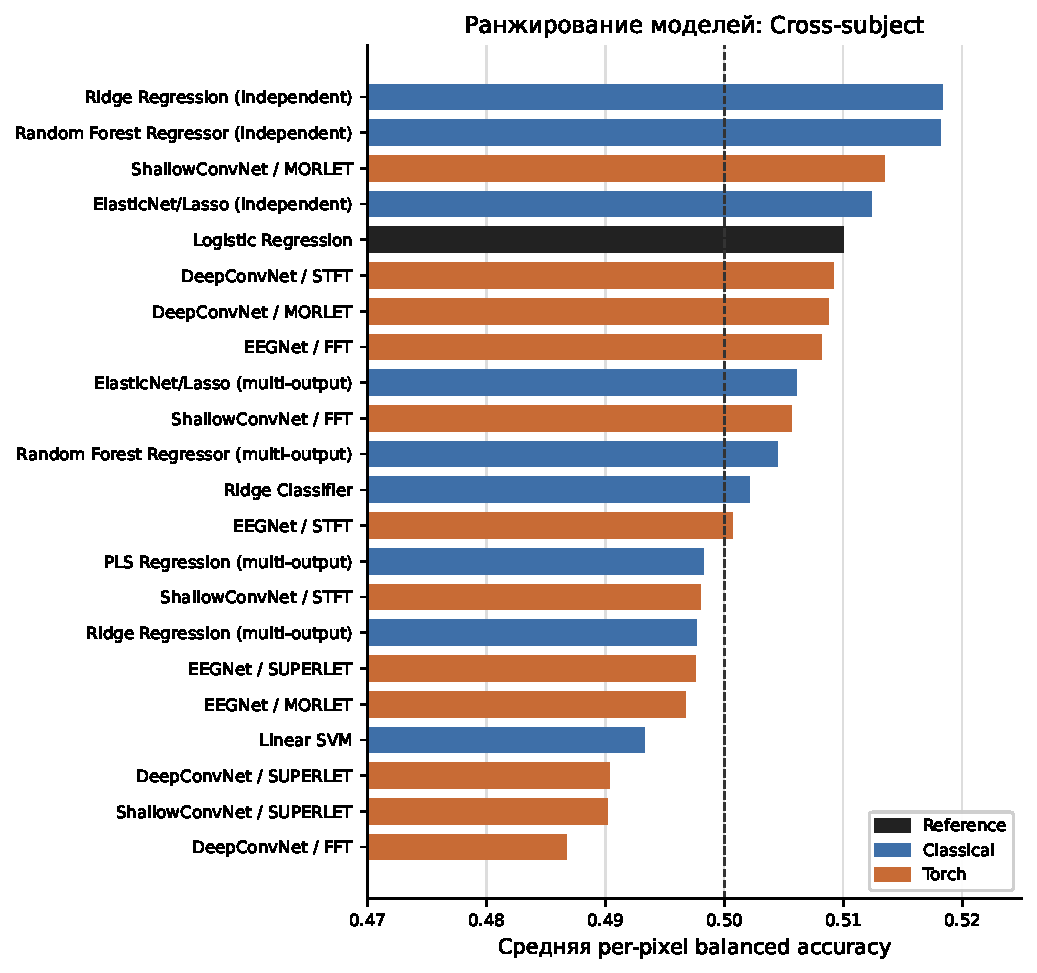
\includegraphics[width=\linewidth,height=0.52\textheight,keepaspectratio]{experiment_cross_subject_ranking.pdf}
      \centering\scriptsize Межсубъектный протокол: Ridge Regression independent, \metric{0.518382} [0.486733; 0.561786].
    \end{column}
    \begin{column}{0.48\textwidth}
      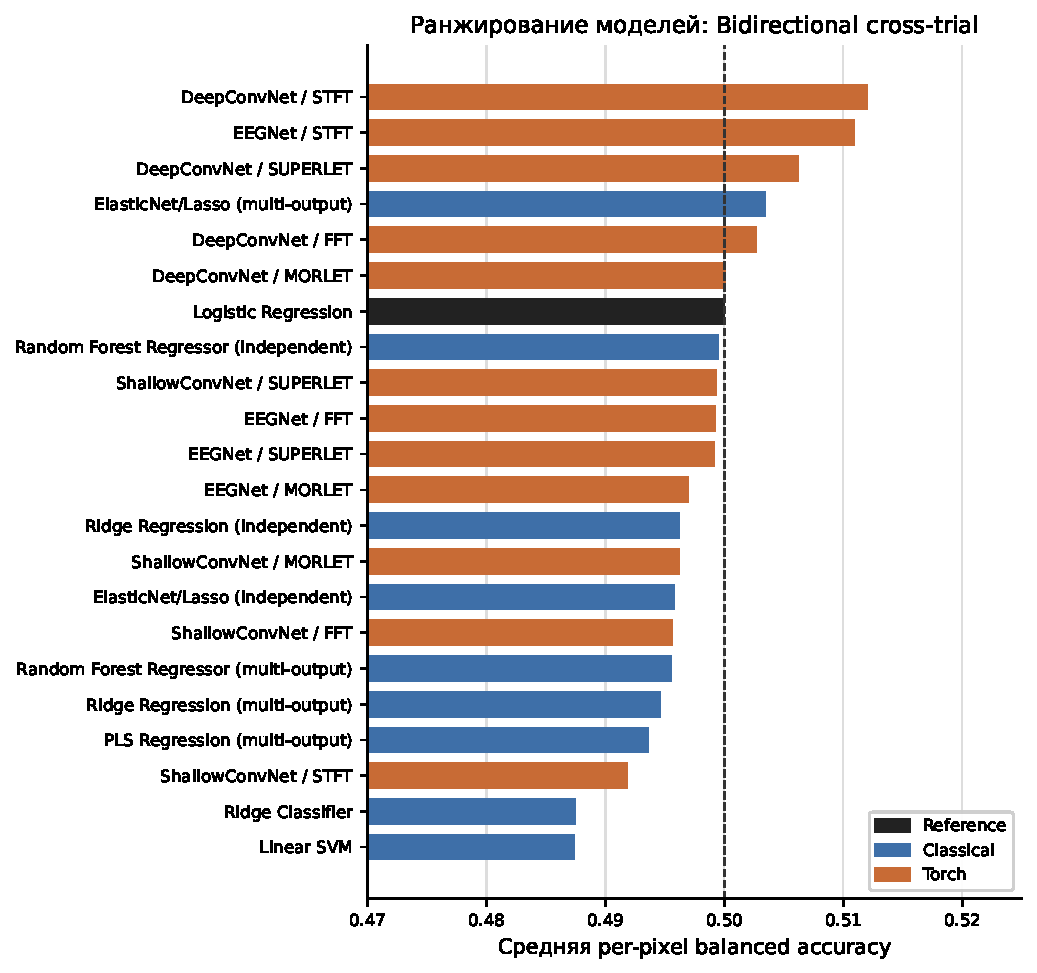
\includegraphics[width=\linewidth,height=0.52\textheight,keepaspectratio]{experiment_within_subject_ranking.pdf}
      \centering\scriptsize Межпробный протокол: DeepConvNet STFT, \metric{0.512011} [0.500668; 0.520872].
    \end{column}
  \end{columns}
  \vspace{0.25em}
  \centering
  \scriptsize
  Оба лидера являются описательными: надежного превосходства над Logistic Regression не обнаружено; минимальное Holm-adjusted $p=0.273000$.
\end{frame}

\begin{frame}{Что видно на отдельных реконструкциях}
  \centering
  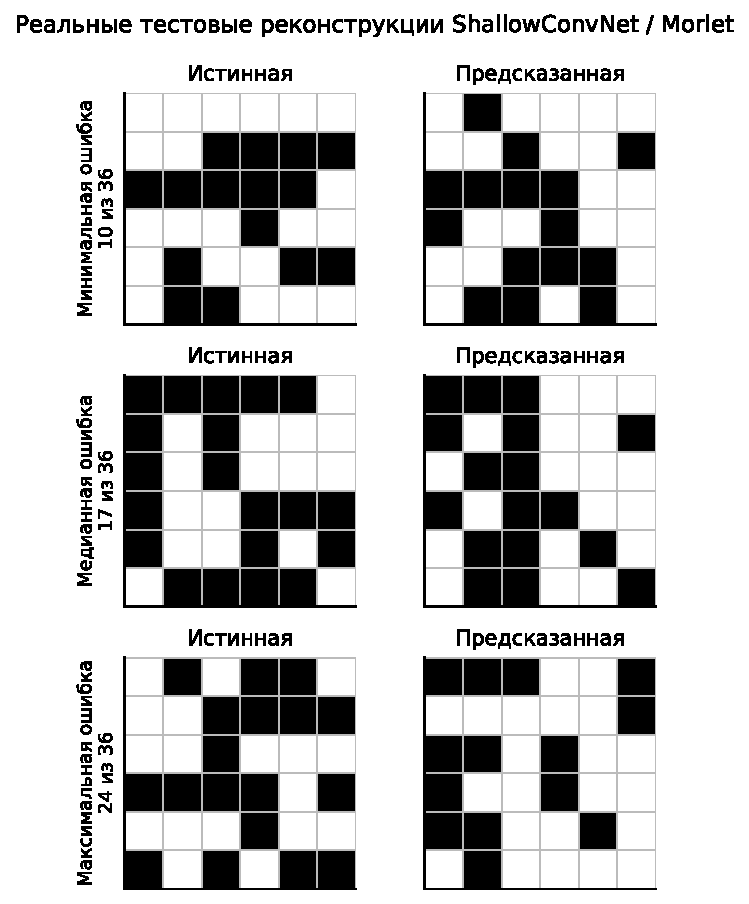
\includegraphics[height=0.70\textheight]{experiment_reconstruction_examples_real.pdf}

  \vspace{0.35em}
  \begin{columns}[T,totalwidth=\textwidth]
    \begin{column}{0.31\textwidth}
      \small Есть отдельные совпадающие пиксели.
    \end{column}
    \begin{column}{0.31\textwidth}
      \small Целая форма обычно не восстанавливается.
    \end{column}
    \begin{column}{0.31\textwidth}
      \small Полное совпадение 36-битного изображения остается редким событием.
    \end{column}
  \end{columns}
\end{frame}

\begin{frame}{Проверка контура на открытых EEG-корпусах}
  \small
  \begin{tabularx}{\textwidth}{@{}lYlY@{}}
    \toprule
    Корпус & Задача & Эпохи & Лучший результат \\
    \midrule
    BNCI2014-001 & 4 класса моторного воображения, LOSO & 5184 & CSP+LDA: \metric{0.385224} при случайном уровне 0.25. \\
    BNCI2014-009 & P300 Target/NonTarget, LOSO & 17280 & ERP/xDAWN Logistic Regression: \metric{0.764062}, macro F1 \metric{0.711260}, ROC AUC \metric{0.850690}. \\
    \bottomrule
  \end{tabularx}
  \vspace{0.8em}
  \begin{block}{Интерпретация}
    Эти эксперименты показывают, что реализованный EEG/ML-контур способен находить сигнал на известных BCI-задачах. Это не внешняя валидация реконструкции случайных $6\times6$ изображений.
  \end{block}
\end{frame}

\begin{frame}{Итог: строгая проверка вместо завышенного вывода}
  \begin{block}{Что сделано}
    Построен воспроизводимый контур реконструкции $6\times6$ стимулов по EEG: 36 бинарных выходов, сравнение классических и CNN-моделей, контроль утечек и сохранение проверяемых артефактов.
  \end{block}

  \vspace{0.25em}
  \begin{columns}[T,totalwidth=\textwidth]
    \begin{column}{0.48\textwidth}
      \begin{block}{Что показали данные}
        \small
        Результаты основной задачи остаются около случайного уровня; надежного превосходства над Logistic Regression не выявлено.
      \end{block}
    \end{column}
    \begin{column}{0.48\textwidth}
      \begin{block}{Почему это важно}
        \small
        Отрицательный результат получен при строгой оценке, а BNCI-проверки показывают работоспособность EEG/ML-контура.
      \end{block}
    \end{column}
  \end{columns}

  \vspace{0.45em}
  \begin{block}{Дальнейшая работа}
    Расширение корпуса, независимая реконструкционная валидация, персональная адаптация, EOG/мультимодальный контроль и transfer learning.
  \end{block}

  \vspace{0.35em}
  \centering
  \textbf{Главный вывод: текущие данные не подтверждают надежную реконструкцию, но задают честную и воспроизводимую основу для следующего эксперимента.}
\end{frame}

\end{document}
